\documentclass[letter, 11pt]{article}
%% ================================
%% Packages =======================
\usepackage[utf8]{inputenc}      %%
\usepackage[T1]{fontenc}         %%
\usepackage{lmodern}             %%
\usepackage[spanish]{babel}      %%
\decimalpoint                    %%
\usepackage{fullpage}            %%
\usepackage{fancyhdr}            %%
\usepackage{graphicx}            %%
\usepackage{amsmath}             %%
\usepackage{color}               %%
\usepackage{mdframed}            %%
\usepackage[colorlinks]{hyperref}%%
\usepackage{wrapfig}             %%
%% ================================
%% ================================

%% ================================
%% Page size/borders config =======
\setlength{\oddsidemargin}{0in}  %%
\setlength{\evensidemargin}{0in} %%
\setlength{\marginparwidth}{0in} %%
\setlength{\marginparsep}{0in}   %%
\setlength{\voffset}{-0.5in}     %%
\setlength{\hoffset}{0in}        %%
\setlength{\topmargin}{0in}      %%
\setlength{\headheight}{54pt}    %%
\setlength{\headsep}{1em}        %%
\setlength{\textheight}{8.5in}   %%
\setlength{\footskip}{0.5in}     %%
%% ================================
%% ================================

%% =============================================================
%% Headers setup, environments, colors, etc.
%%
%% Header ------------------------------------------------------
\fancypagestyle{firstpage}
{
  \fancyhf{}
  \lhead{
\includegraphics[height=4.5em]{LogoDFI.jpg}}
  \rhead{FI3104-1 \semestre\\
         Métodos Numéricos para la Ciencia e Ingeniería\\
         Prof.: \profesor}
  \fancyfoot[C]{\thepage}
}

\pagestyle{plain}
\fancyhf{}
\fancyfoot[C]{\thepage}
%% -------------------------------------------------------------
%% Environments -------------------------------------------------
\newmdenv[
  linecolor=gray,
  fontcolor=gray,
  linewidth=0.2em,
  topline=false,
  bottomline=false,
  rightline=false,
  skipabove=\topsep
  skipbelow=\topsep,
]{ayuda}
%% -------------------------------------------------------------
%% Colors ------------------------------------------------------
\definecolor{gray}{rgb}{0.5, 0.5, 0.5}
%% -------------------------------------------------------------
%% Aliases ------------------------------------------------------
\newcommand{\scipy}{\texttt{scipy}}
%% -------------------------------------------------------------
%% =============================================================
%% =============================================================================
%% CONFIGURACION DEL DOCUMENTO =================================================
%% Llenar con la información pertinente al curso y la tarea
%%
\newcommand{\tareanro}{04}
\newcommand{\fechaentrega}{15/09/2019 23:59 hrs}
\newcommand{\semestre}{2019B}
\newcommand{\profesor}{Valentino González}
%% =============================================================================
%% =============================================================================


\begin{document}
\thispagestyle{firstpage}

\begin{center}
  {\uppercase{\LARGE \bf Tarea \tareanro}}\\
  Fecha de entrega: \fechaentrega
\end{center}


%% =============================================================================
%% ENUNCIADO ===================================================================
\noindent{\large \bf Problema}

\begin{wrapfigure}{r}{0.6\textwidth}
  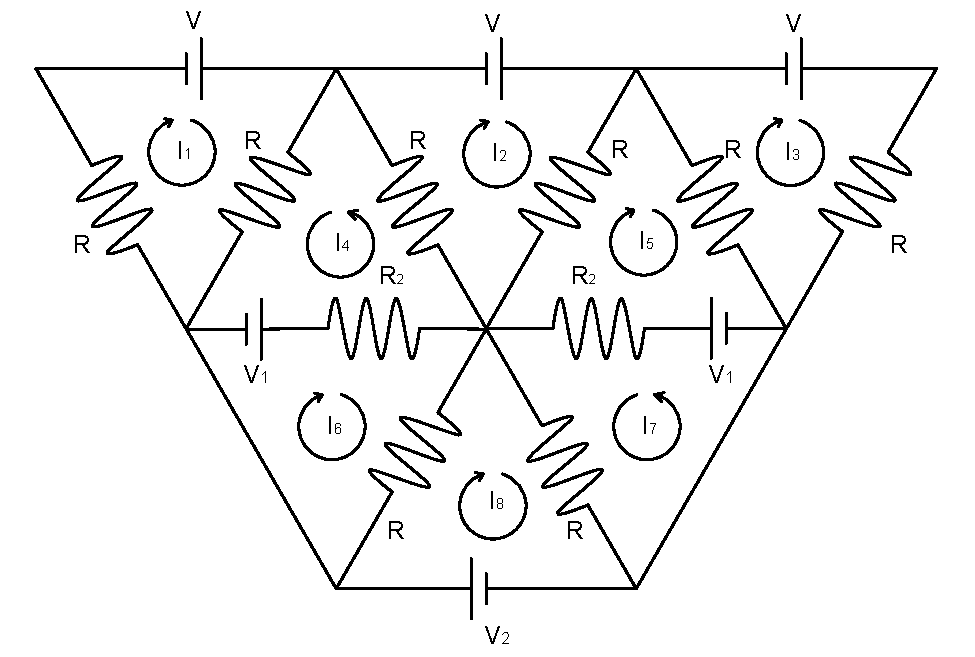
\includegraphics[width=0.58\textwidth]{circuit.pdf}
\end{wrapfigure}

Considere el circuito de la figura. Todas las resistencias que aparecen
dibujadas oblicuas son R=4$\Omega$ mientras que las horizontales son
R$_2$=3$\Omega$. Las fuentes de voltage tienen valores V=20V, V$_1$=30V y
V$_2$ es una fuente variable. El circuito es tal que se quema si alguna de las
corrientes pasando por el circuito supera los 20 amperes (el problema no es
necesariamente muy realista).

Determine el valor máximo que puede tener V$_2$ de modo que el sistema no se
queme.


\vspace{2em}
¿Cómo resolver el problema?
\vspace{1em}

Ud. debe escribir la ecuación de Kirchoff para circuitos ($V=R\times I$) para
cada uno de los circuitos elementales cerrados que componen el circuito más
complejo (es decir, cada uno de los triángulos en el dibujo). Al hacerlo, Ud.
obtendrá un sistema de 8 ecuaciones para 8 incógnitas (las corrientes
$I_{1-8}$). Escriba este sistema de ecuaciones de forma matricial de modo que
se pueda expresar como:

$$
R \times \vec{I} = \vec{V}
$$

\noindent donde $R$ es una matriz de 8$\times$8 e $\vec{I}$ es el vector de las
corrientes, $(I_1, ..., I_{8})^t$.

\begin{ayuda}
  \small
  \noindent {\bf Ayuda.}
  Si no está familiarizado con cómo hacer este tipo de análisis, hay varios
  videos en \texttt{youtube} que le pueden ayudar. Por ejemplo
  \href{https://www.youtube.com/watch?v=DPNuiyi6XLQ&t=131s}{este}, pero hay
  muchos que le pueden ayudar.
\end{ayuda}


Para V$_2$ explore el rango de valores 10V -- 30V, variando V$_2$ y calculando
la corriente máxima que pasa por el circuito cada vez (por simplicidad sólo
preocupese del valor máximo del vector $\vec{I}$ y recuerde que lo importante
es el valor absoluto de cada uno de sus elementos).

Ahora utilice algún algoritmo de búsqueda de ceros para encontrar el valor de
V$_2$ para el cual el circuito se quema.

\vspace{0.5em}
\noindent{\large \bf Requerimiento.}
Se pide que elija un método para la búsqueda de ceros y para ese mismo método
compare dos alternativas para resolver el sistema de ecuaciones. Por ejemplo,
dado que la matriz R no cambia al cambiar V$_2$, Ud. podría intentar una
descomposición PLU de la matriz R y utilizarla en el algoritmo de busqueda de
ceros. Otra alternativa podría ser invertir cada vez la matriz. Por último, la
matriz R no esta densamente poblada por lo que podría intentar alguno de los
algoritmos para \texttt{sparse matrices}, sea creativo. Compare los dos
mecanismos elegidos en términos de tiempo de ejecución y discuta sobre las
diferencias observadas.

% \vspace{1em}
\pagebreak
\noindent{\bf Instrucciones importantes.}
\begin{itemize}

  \item Utilice \texttt{git} durante el desarrollo de la tarea para mantener un
    historial de los cambios realizados. La siguiente
    \href{https://education.github.com/git-cheat-sheet-education.pdf}{cheat
      sheet} le puede ser útil. \textbf{Esta vez revisaremos el uso apropiado
    de la herramienta y asignaremos una fracción del puntaje a este ítem.}
    Realice cambios pequeños y guarde su progreso (a través de \emph{commits})
    regularmente. No guarde código que no corre o compila (si lo hace por algún
    motivo deje un mensaje claro que lo indique). Escriba mensajes claros que
    permitan hacerse una idea de lo que se agregó y/o cambió de un
    \texttt{commit} al siguiente.

  \item También comenzaremos a revisar su uso correcto de \texttt{python}. Si
    define una función relativametne larga o con muchos parámetros, recuerde
    escribir el \emph{docstring} que describa los parámetros que recibe la
    función, el output, y el detalle de qué es lo que hace la función. Recuerde
    que generalmente es mejor usar varias funciones cortas (que hagan una sola
    cosa bien) que una muy larga (que lo haga todo).  Utilice nombres
    explicativos tanto para las funciones como para las variables de su código.
    El mejor nombre es aquel que permite entender qué hace la función sin tener
    que leer su implementación.

  \item Para \texttt{python} existe una guía de estilo sintáctico
    (\texttt{PEP8}) que entrega un set de reglas simples para crear código
    ordenado y fácilmente legible por otras personas. Por ejemplo, se
    recomienda no usar lineas más largas que 79 caracteres. En el futuro
    revisaremos que su código apruebe \texttt{pep8}, por ahora le sugerimos que
    lea la guía \href{https://www.python.org/dev/peps/pep-0008/}{acá} se
    familiarice con las reglas y trate de implementarlas en esta tarea a modo
    de ejercicio. En \href{http://pep8online.com}{esta página} puede chequear
    si su código aprueba \texttt{PEP8}. También hay utilidades en la línea de
    comando que permiten hacer la prueba directamente en sus computadores: 
    
    \texttt{>\ pip install pycodestyle}\\
    \texttt{>\ pycodestyle <filename>}

  \item La tarea se entrega subiendo su trabajo a github. Cuando termine
    asegúrese de hacer un último \texttt{commit} y luego un \texttt{push} para
    subir todo su trabajo a github.

  \item El informe debe ser entregado en formato \texttt{pdf}, este debe ser
    claro sin información de más ni de menos. \textbf{Esto es muy importante,
    no escriba de más, esto no mejorará su nota sino que al contrario}. Por
    ejemplo, la presente tarea probablemente no requiere informes de más de 4
    páginas en total (esto no es una regla estricta, sólo una referencia útil).
    Asegúrese de utilizar figuras efectivas y tablas para resumir sus
    resultados. Revise su ortografía.

  \item Repartición de puntaje: 50\% implementación y resolución del problema
    (independiente de la calidad de su código); 40\% calidad del reporte
    entregado: demuestra comprensión del problema y su solución, claridad del
    lenguaje, calidad de las figuras utilizadas; 5\% uso apropopiado de
    \texttt{git}; 5\% diseño del código: modularidad, uso efectivo de nombres
    de variables y funciones, docstrings, etc.

\end{itemize}

%% FIN ENUNCIADO ===============================================================
%% =============================================================================

\end{document}
